\section{Adding data or opening an existing file}

    When opening the GUI, a temporary HDF5 file is automatically created in a temporary folder. From there, you can either populate this temporary file with data or open another non-temporary file. In both cases, you can choose to add data or open an existing file a few different ways:
    \begin{itemize} 
        \item Drag and drop your data or a file into the left pannel.
        \item Click on the "Open" (respectively "Add data") button in the toolbar to select a file from your filesystem
        \item To add data, you can also right-click on the left pannel and select "Add data" to select a file from your filesystem.
    \end{itemize}

    Note that all these methods are equivalent and will achieve the same result. Their use is a matter of personal preference.

\section{Visualizing the structure of the file}

    Once a file is opened or data is added, the left pannel will display the structure of the HDF5 file. This structure is organized in a tree format, where each node represents a group or dataset within the HDF5 file. You can expand or collapse these nodes to navigate through the hierarchy of your data.

    \begin{figure}[H]
        \centering
        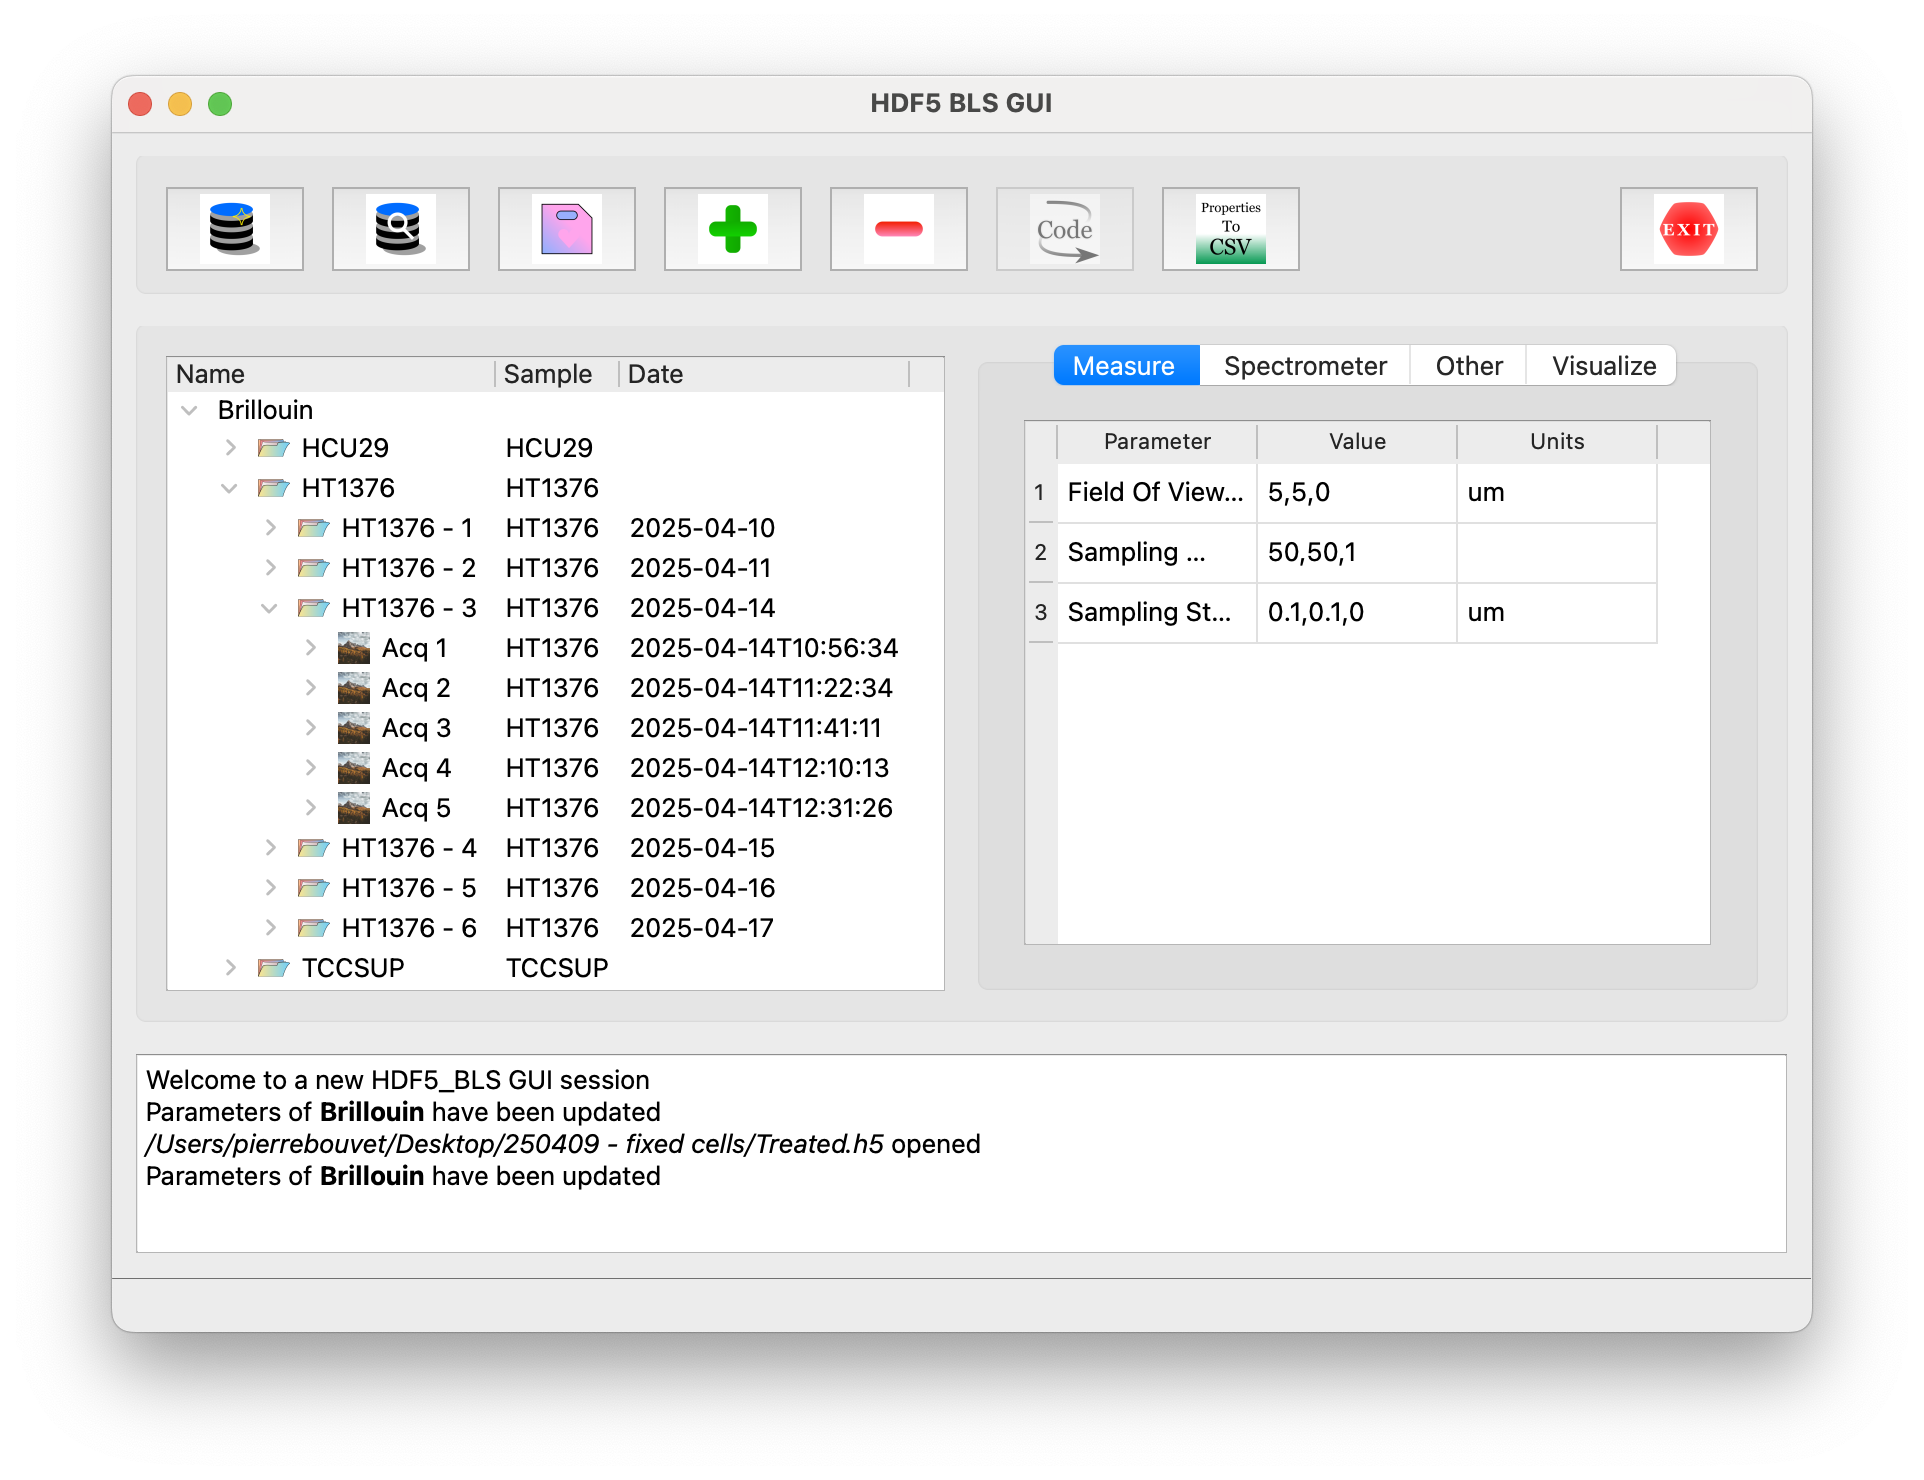
\includegraphics[width=\textwidth]{img/main_window_hierarchy.png}
        \caption{HDF5\_BLS\_GUI Main Window with an opened file}
        \label{fig:gui_main_window_hierarchy}
    \end{figure}